\section{A lens modeling challenge} \label{sec:results}

% \subsection{\sw} \label{sec:SpaceWarps} some words about \sw

Interested volunteers from the \sw forum were initially introduced to
\spl through a video tutorial and by videocon.  After this
introductory stage, a modelling challenge was presented.  This
consisted of 29 simulated lenses (sims) covering a range of lensing
configurations.

\subsection{The simulated lenses} \label{sec:sims}

The sims were generated by AM, in consultation with PM and AV.  In the
interest of blind testing, the information in this section was
revealed neither to RK, while choosing the challenge set, nor to the
people making models (EB, CC, CM, JO, PS and JW) until they were done.

The sims produced using {\tt gravlens}
\citep{2001astro.ph..2341K,2001astro.ph..2340K} and were of three
kinds, as follows.

\begin{itemize}
  \item {\em Quasar:\/} A singular elliptical isothermal plus constant
    external shear, with a circular Gaussian source.
  \item {\em Galaxy:\/} Lens as with quasar, but elliptical de
    Vaucouleurs source.
  \item {\em Galaxy:\/} Lens is circular NFW plus one dominant
    elliptical SIE and perturbating elliptical SIEs, source as with
    galaxy.
\end{itemize}

Singular isothermal is in equations (33-35) of
\cite{2001astro.ph..2341K} with core radius set to zero. NFW is
equations (48,50) of the same paper, and shear is the $\gamma$ term in
equation (76) of that work.

\subsection{Some example models}

Figure \ref{fig:6941} shows a simple example.

Figure \ref{fig:6975} shows an example where substructure introduces a
complication, but model ok.

Figure \ref{fig:6937} shows a case where substructure leads to a
poorer model.

Figure \ref{fig:6975} shows a nice symmetric quad.

Figure \ref{fig:6990} shows a long-axis quad.

Figure \ref{fig:6919} shows a short-axis quad.

Figure \ref{fig:6915} shows an inclined quad.

Figure \ref{fig:6971} shows incorrect identification, but the enclosed
mass still quite well recovered.


\subsection{The test setup} \label{sec:testsetup}

To estimate the performance of the volunteers and the quality of the generated models, two test T1 and T2 were done.
%\begin{enumerate}
%  \item (T1) Correct identification of extremal points
%  \item (T2) Reproduction of the mass distribution of the lens
%\end{enumerate}

T1 tested the volunteers ability to reconstruct the arrival time surface given a survey image containing a sim.
This task consists of two parts.
First, the correct identification and location of lensed images (T1a).
Second to find the correct ordering in respect of the arrival time for the identified lensed images (T1b).

While we expected T1a to be trivial, given the nature of the survey images and the success of \sw, we expect T1b to pose more problems.
T1b tests the volunteers understandings of the theory of arrival time surfaces and the odd number theorem.
While we can provide the volunteers with some general rule of thumbs, T1b involves imagination and guessing and therefore training could improve their skills in a later stage.

T1 was also designed to give some feedback on the difficulties volunteers encounter, to further imrove the tutorial materials.

The second test T2 was to compare the desired results of a modeling process, the mass distribution of the lens $\kappa(x, y)$.
To get a means of comparing the simulated data (sims) to the generated modeled data (models), the total convergence, also called enclosed mass $\kappa_{\text{encl}}(r)$ for both was calculated.
The Einstein radius $\Theta_E$ is defined by $\kappa_{\text{encl}}(\Theta_E)=1$ and gives a number that allows the comparison between the sims and the models.
We also let an expert model two selected systems to compare the results from volunteers to those of a professional.

\todo{!} Should I write down prior expectation for T2 too?




\subsection{First test T1} \label{sec:tests.t1}

The evaluation of the volunteers performance for T1 was done manually, comparing their input from \spl and the resulting reconstructed arrival time surface contour line plot (arrival plot) to the arrival plot genreated using simulation parameters.
\Figref{output_compare} shows the setup used to evaluate the models.

\begin{figure}
  \centering
  \subfigure{\includegraphics[width=0.45\textwidth]
             {fig/sims/006917/input.png}}
  \subfigure{\includegraphics[width=0.45\textwidth]
             {fig/sims/006917/spaghetti.png}} \\
  \subfigure{\includegraphics[width=0.45\textwidth]
             {fig/sims/ASW0001hpf/arriv.png}}
%  \subfigure{\includegraphics[width=0.45\textwidth]
%             {fig/sims/ASW0001hpf/extr_points.png}}
  \caption{Examples of Spaghetti input (left top) and modeled arrival time surface (right top) vs reconstructed arrival time surface from simulation parameters (bottom).}
  \label{fig:output_compare}
\end{figure}

To evaluate T1a and T1b, each model was evaluated with two binary tests.
The first is passed, if all the images have been identified and are approx. within $\pm0.05\cdot\text{imgage width}$.
The second test is passed, if those identified points have the right parity, ordering with respect to arrival time.

Additionally, ten types of errors that could occur were analyzed, where each model could contain multiple of those.
The complete table with the results for each model can be found in the appendix, \tabref{detail_results}.


%\begin{enumerate}
%1  \item inaccurate placement in an extended arc
%2  \item wrongly identified sad and min in 3 image configuration
%3  \item identified only 3 instead of 5 images
%4  \item tried to model an arc with a min instead of min-sad-min
%5  \item PI-err (rotation by 180 degrees; in 5 image configuration, exchanged the ordering of the two saddle points)
%6  \item PI/2-err (rotation by 90 degree; sad$\longmapsto$min$\longmapsto$sad$\longmapsto$min$\longmapsto$sad)
%7  \item missed faint image(s)
%8  \item tried to model an arc with min-sad-min instead of only min
%9  \item did identify two close by images as one
%10  \item used 7 or more image to model a 5 image system.
%\end{enumerate}

\input{tab/auto/_stats}

In \tabref{stats} a summary of this evaluation is presented.
We conclude that the volunteers are performing very well identifying and positioning images (T1a), with a performance of 92\% (R1 p=0.92).
Most of the problems where due to unclear arc-like structures (E01, p=0.18; E04, p=0.03; E08, p=0.04).
Critical failures like the failure to identify all five images in an five image system (E03, p=0.04) or to include too many images (E10, p=0.01) did almost never happened.
From this we conclude that the introduction materials was adequate and the volunteers understand the basics of gravitational lensing.

\todo{add more detail?} Add more details like total amount of images detected / tot am images (rightPlace fraction)??

The assignment of the parity of the images (T1b) posed a more difficult task.
In 59\% (R2, p=0.59, N=70) of the cases the volunteers succeeded to identify the right configuration.
Most of the failures are due to E06, with N=38, p=32\%, followed by E05 (PI) with N=7, p=6\%.
For an example of E06, see \figref{6971}, it basically describes a situation, where the minima and saddlepoints were exchanged (rotated by $\pm90\dgr$).
E05 describes the situation, where the ordering of the saddle points was wrong (rotation by $180\dgr$)
While these errors occurred, we suspect they can be avoided with better training material and some examples for the obvious cases.
For more challenging cases, like very symmetrical distribution of the lensed images (for example model 6971, \figref{6971}), those errors should still produce plausible results, as will be explained in the next section.







\subsection{Second test T2} \label{sec:results.2}

To compare the enclosed mass profile and the Einstein radius of the simulation and the models, \kenc was calculated using the mass map \kap[x,y] directly generated in the modeling process.
From the ensemble of models generated by one modeling process, the mean is taken as the resulting $\kappa(r)$ to calculate $\theta_E$.
To estimate the errors, also the extremal models are used to estimate a lower and upper limit for $\theta_E$.
These results can be seen in \figref{eR_all_models}.
This figure shows that this technique of estimating the error is underestimating the error significantly and should be improved for further analysis.

\begin{figure}[htbp]
  \centering
    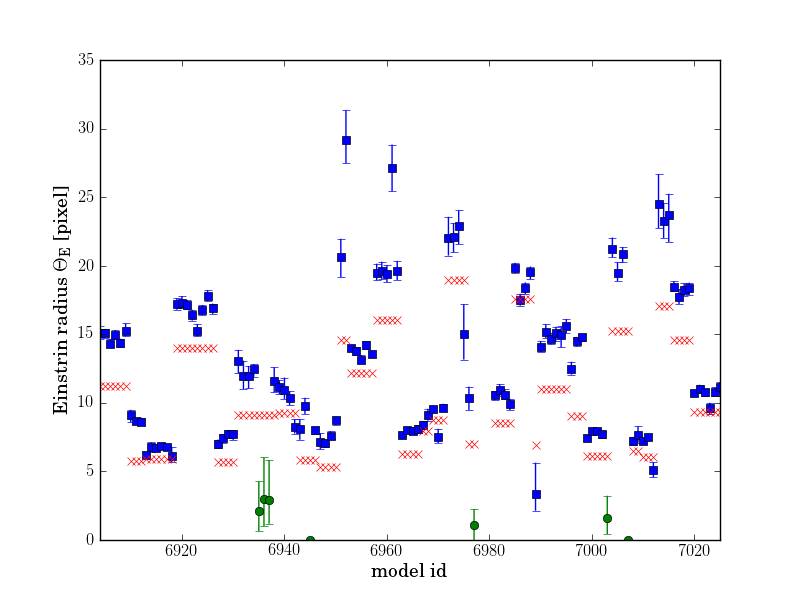
\includegraphics[width=0.80\textwidth]{fig/sims/eR_1.png}
  \caption{\tEr \gEr for all models with estimated errors in blue squares, \gEr of simulation in red crosses}
  \label{fig:eR_all_models}
\end{figure}

In \figref{eR_per_sim} can be seen, that the calculated \tEr \gEr of the models tend to be too high.
The overshoot varies from around 0.2 to 0.4 for for good models.
One of the reasons for this is, that it's hard to get the center of the lens on spot.
An offset leads to a a flatter mass profile for the model compared to the simulation.



\begin{figure}[htbp]
  \centering
    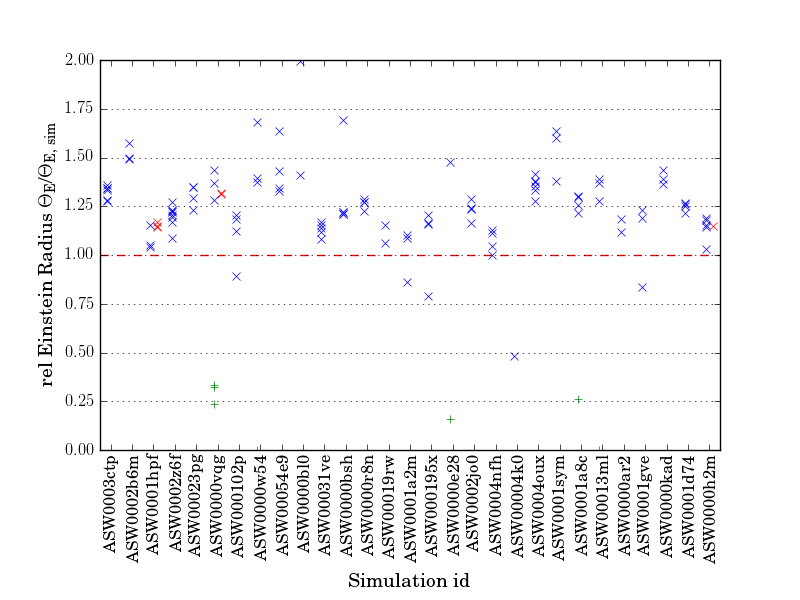
\includegraphics[width=0.80\textwidth]{fig/sims/eR_4.png}
  \caption{relative Einstein Radius \gEr / \gEr[, sim] for each model, per sim. red crosses with right offset for models made by an expert.}
  \label{fig:eR_per_sim}
\end{figure}


Error 5 and 6 happen mostly in very symmetric images, where it's hard to tell
It changes the orientation of the mass distribution \kap[x,y].
But \kenc and thus the \tEr \gEr is not changed, and thus the final result is still a valid model.
This can be seen by comparing the results for \asw{0h2m}, shown in \figref{kapenc_compare_faulty}: 
The correct model 7022 ($\mEr=10.76$), which was done by an expert, and
7020 ($\mEr=10.72$),
7024 ($\mEr=10.80$),
7025 ($\mEr=11.16$),
7021 ($\mEr=11.04$).
The first three show error 6, while the last is of error type 5.
This can be easily corrected, if further analysis is done for the modeled system and time delays are known.

\begin{figure}
  \centering
  \subfigure{\includegraphics[width=0.45\textwidth]
             {fig/sims/007020/kappa_encl}}
  \subfigure{\includegraphics[width=0.45\textwidth]
             {fig/sims/007021/kappa_encl}} \\
  \subfigure{\includegraphics[width=0.45\textwidth]
             {fig/sims/007024/kappa_encl}}
  \subfigure{\includegraphics[width=0.45\textwidth]
             {fig/sims/007025/kappa_encl}}
  \subfigure{\includegraphics[width=0.45\textwidth]
             {fig/sims/007022/kappa_encl}}
  \caption{\kenc for models of \asw{0vqg}: 7020 (top left), 7021 (top right), 7024 (mid left), 7025 (mid right) by volunteers and a correct model 7022 (bottom) by an expert.}
  \label{fig:kapenc_compare_faulty}
\end{figure}

Comparing the models of volunteers and experts can be done in \figref{kapenc_compare_faulty}, where only the
expert got the right configuration, but all the resulting models are comparable, besides rotation.

Two additional sims were modeled by an expert, \asw{1hpf} and \asw{0vqg}.
Looking at the results for \gEr for those models in \figref{eR_per_sim}, we conclude that the performance of volunteers (blue crosses) and experts (red crosses, offset) is comparable.
Please note that the models of \asw{0vqg} with \gEr{, rel} around 0.25 (6935 -- 6937) are failed models that show the attempts of a single user, that came finally up with model 6938 as final result.\todo{remove?}

\clearpage
